%!TEX root = ../report.tex
\documentclass[../report.tex]{subfiles}
\begin{document}
    \chapter{Contributions}\label{ch_contributions}
    \begin{itemize}
    \item Attribution maps presented in the publication \cite{brand2022next}.
      \begin{figure}[H]
      	\centering
      	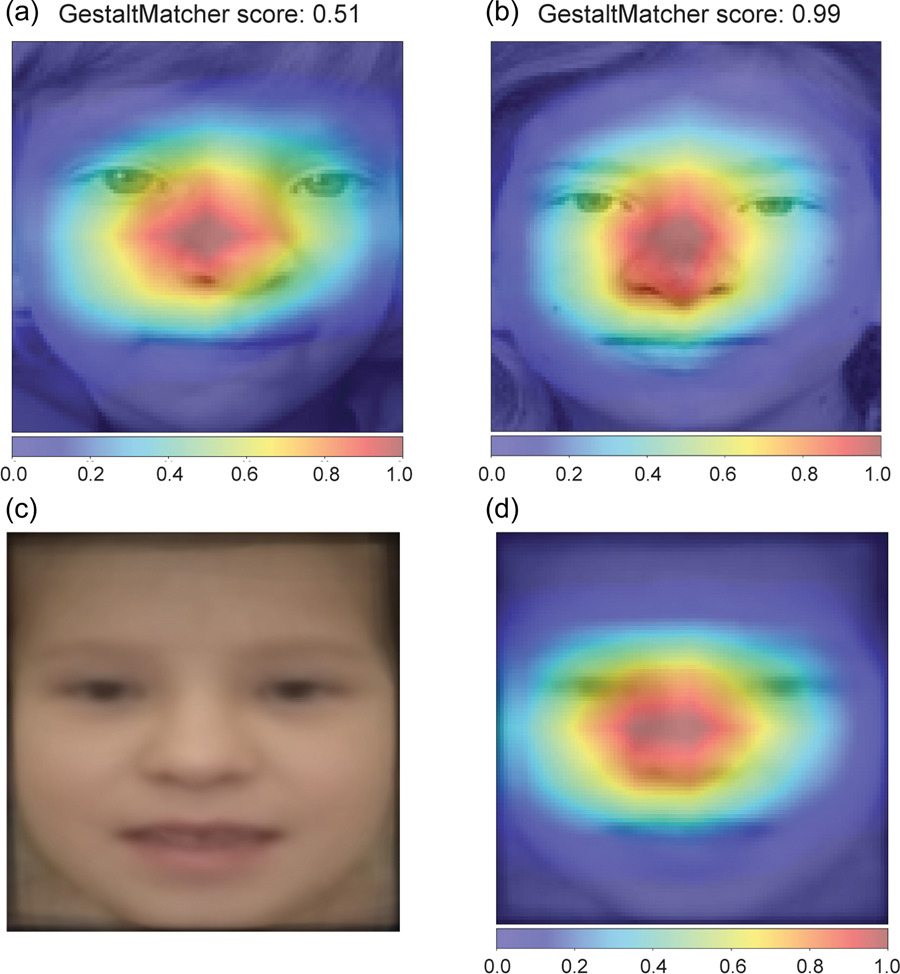
\includegraphics[scale=0.4]{images/kdvs.jpg}
      	\caption{The pixel attribution maps for the Koolen-de Vries syndrome (KdVS) class and the composite face of KdVS. Pixel attribution maps of (a) patient at the age of 8; (b) patient at the age of 15; (c) KdVS composite face. (d) the composite face of KdVS. Attribution maps show the prominence of the nose region for the classifier's prediction. Attribution maps of the patient's photos show high similarity with that of the composite face. The GestaltMatcher score ranges from 0 to 1. The value of one is the highest value indicating high similarity to the disorder}
      \end{figure}
  	\item Research poster presented at AGDev 2022.
      \begin{sidewaysfigure}
    	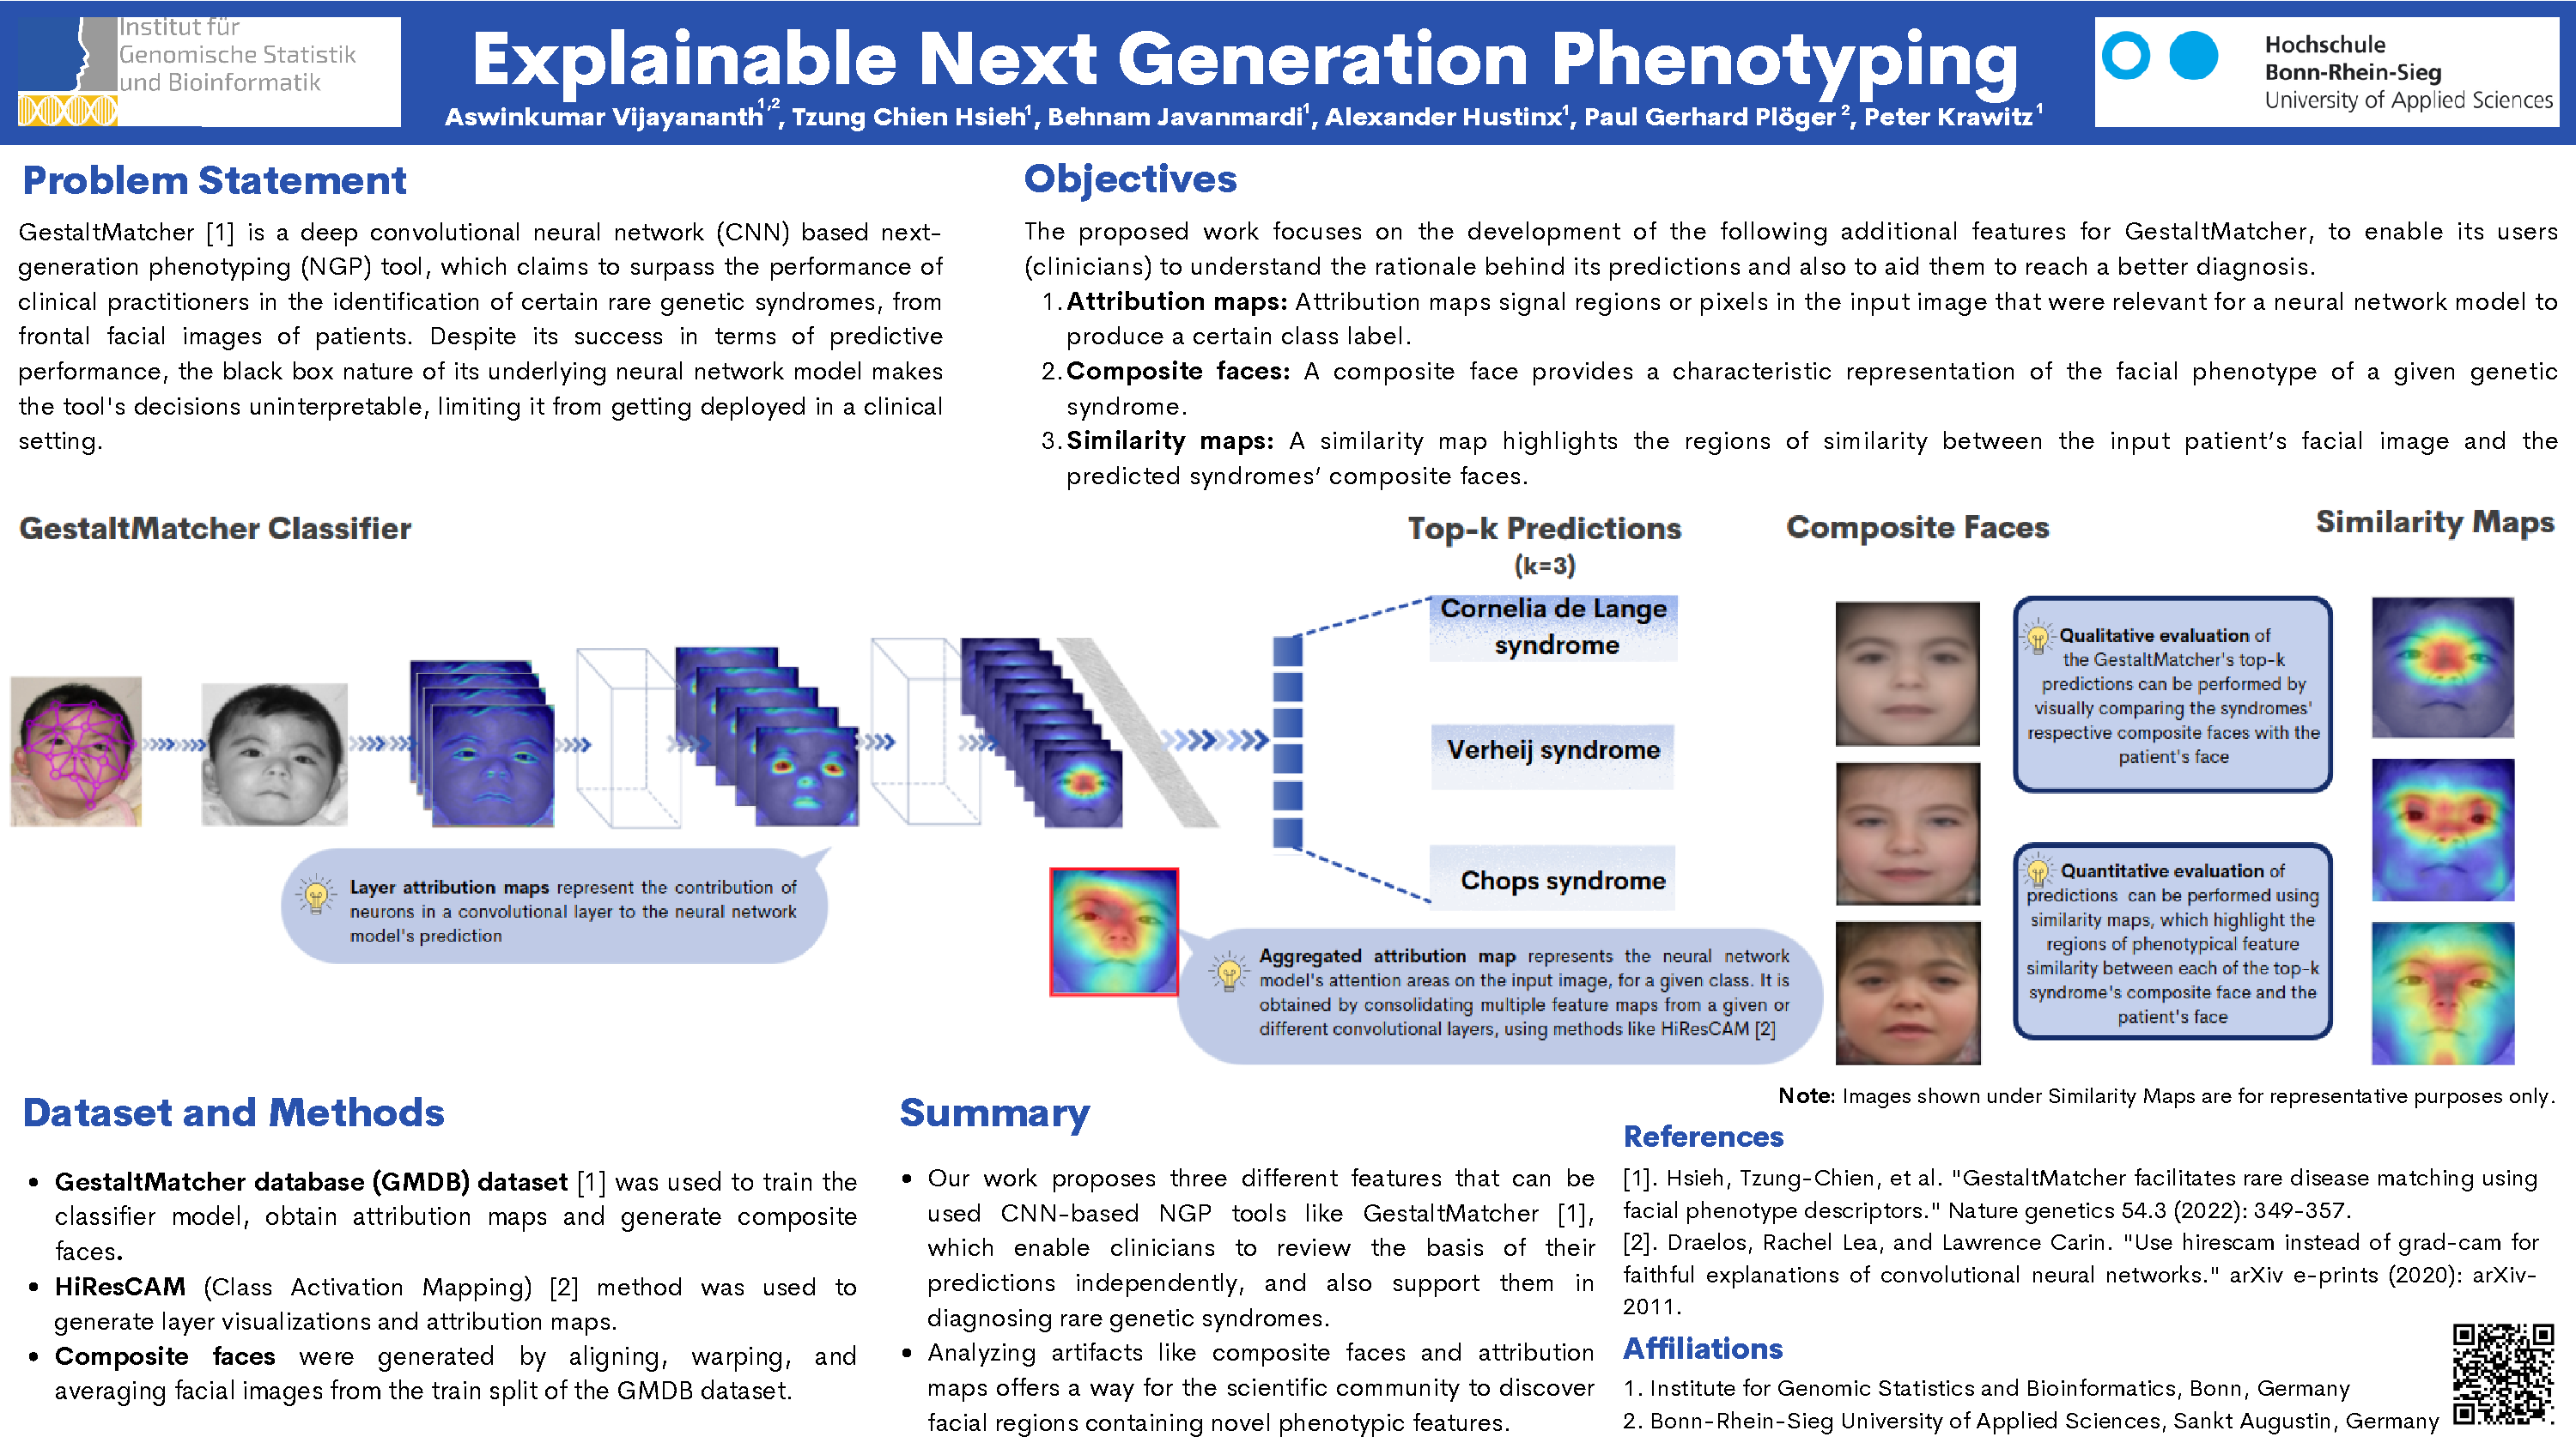
\includegraphics[scale=0.4]{images/poster_1.pdf}
    	\caption{Research poster presented at AGDev2022}
      \end{sidewaysfigure}
	\end{itemize}
    \chapter{Classifer Performance} \label{ch_class_perf}
    \begin{figure}[H]
    	\centering
    	\begin{subfigure}[b]{0.45\textwidth}
    		\centering
    		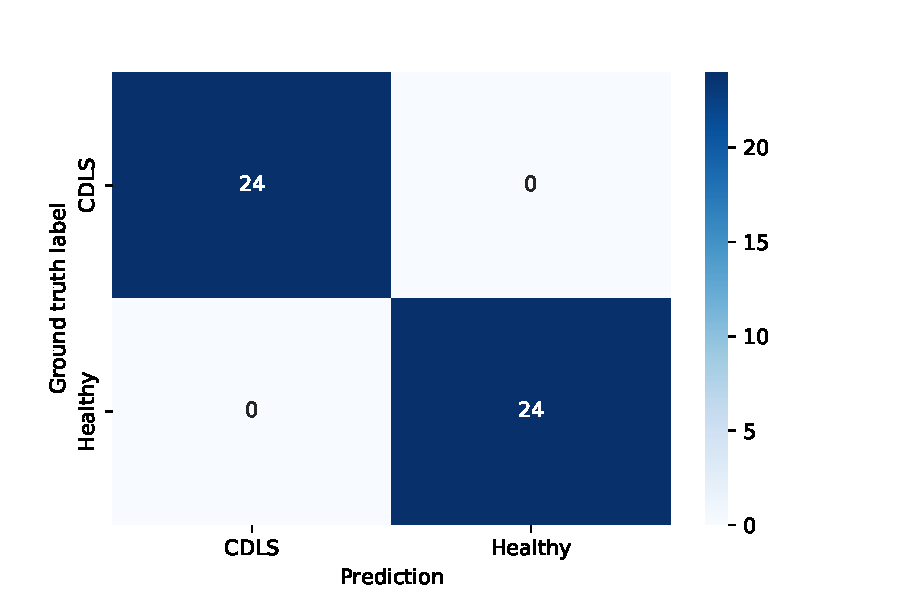
\includegraphics[width=\textwidth]{images/class_0n_conf.pdf}
    		\caption{GC1}
    	\end{subfigure}
    	\begin{subfigure}[b]{0.45\textwidth}
    		\centering
    		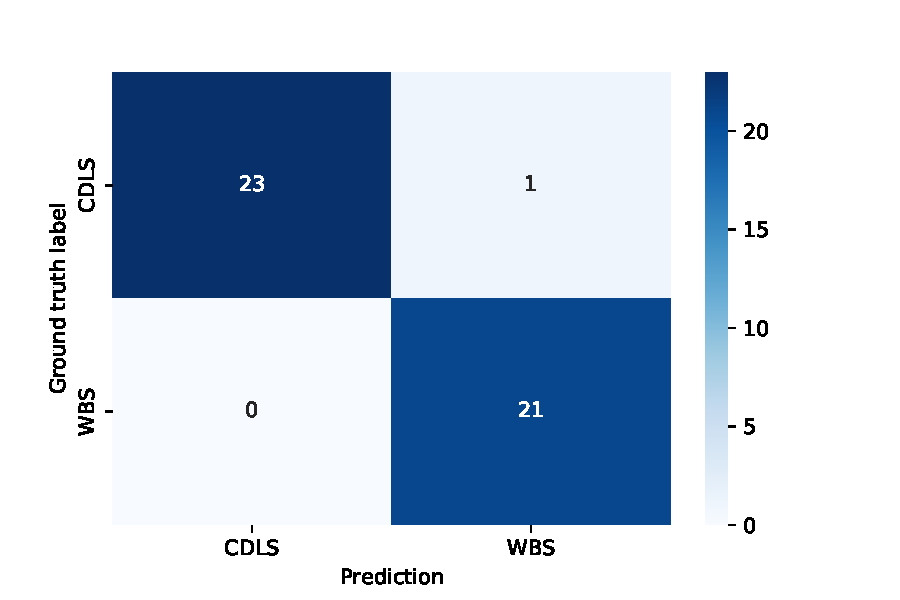
\includegraphics[width=\textwidth]{images/class_01_conf.pdf}
			\caption{GC2}
    	\end{subfigure}
    	\begin{subfigure}[b]{0.45\textwidth}
    		\centering
    		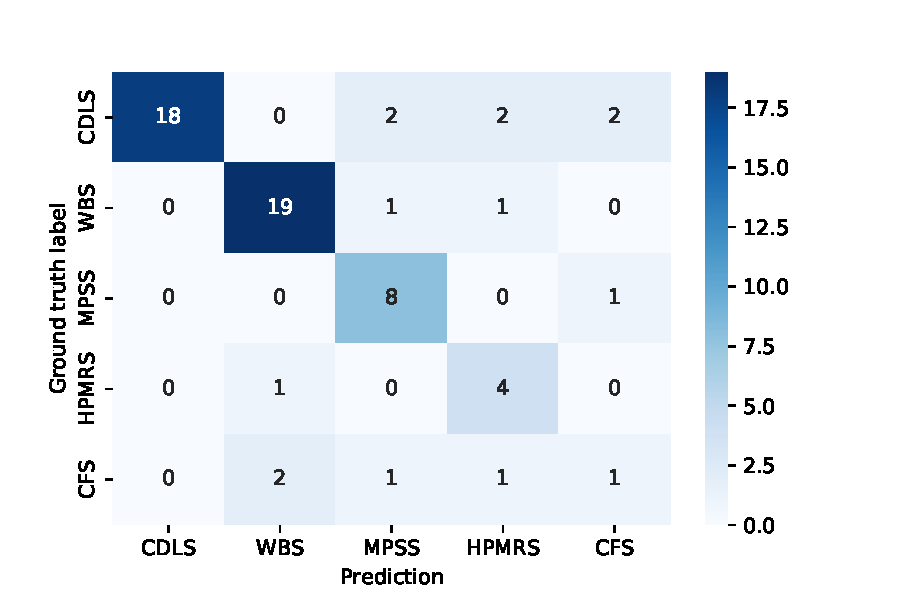
\includegraphics[width=\textwidth]{images/class_b_conf.pdf}
    					\caption{GC3}
    	\end{subfigure}
    	\begin{subfigure}[b]{0.45\textwidth}
    		\centering
    		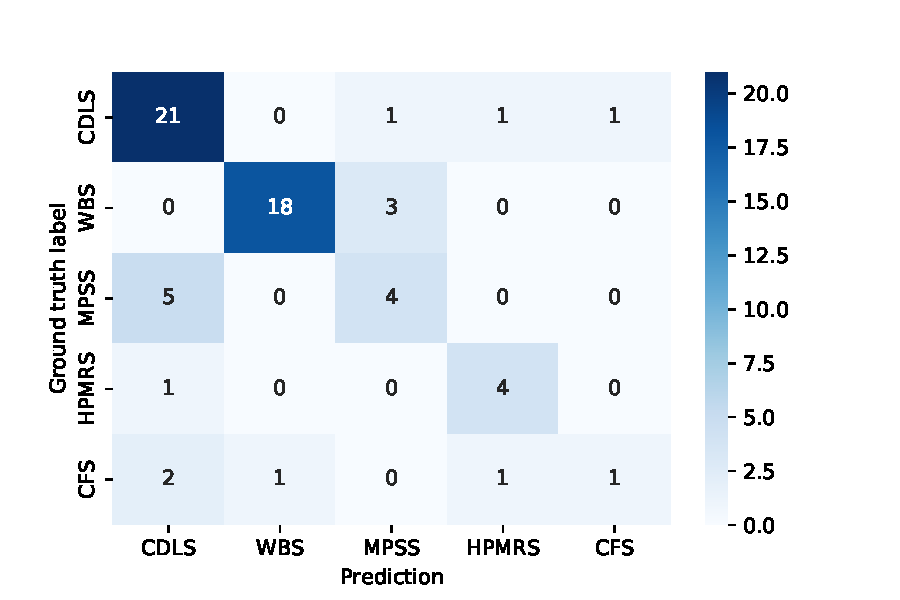
\includegraphics[width=\textwidth]{images/class_i_conf.pdf}
    					\caption{GC4}
    	\end{subfigure}
    \caption{Confusion matrices of the classifier models used for the dataset imbalance - explanation quality experiment}
	\end{figure}

	\begin{table}[H]
		\centering
		\begin{tabular}{|c|c|l|c|c|}
			\hline
			Class   & Test sample count & Precision & Recall & F1-score \\ \hline
			CDLS    & 24                & 1.00      & 1.00   & 1.00     \\ \hline
			Healthy & 24                & 1.00      & 1.00   & 1.00     \\ \hline
		\end{tabular}
	\caption{Test performance of GC1 model}
	\end{table}

	\begin{table}[H]
		\centering
		\begin{tabular}{|c|c|l|c|c|}
			\hline
			Class & Test sample count & Precision & Recall & F1-score \\ \hline
			CDLS  & 24                & 1.00      & 1.00   & 0.98     \\ \hline
			WBS   & 21                & 0.95      & 0.95   & 0.98     \\ \hline
		\end{tabular}
	\caption{Test performance of GC2 model}
	\end{table}
	\begin{table}[H]
		\centering
		\begin{tabular}{|c|c|c|c|c|}
			\hline
			Class & Test sample count & Precision & Recall & F1-score \\ \hline
			CDLS  & 24                & 1.00      & 1.00   & 1.00     \\ \hline
			CFS   & 5                 & 0.25      & 0.20   & 0.22     \\ \hline
			HPMRS & 5                 & 0.50      & 0.80   & 0.62     \\ \hline
			MPSS  & 9                 & 0.67      & 0.89   & 0.76     \\ \hline
			WBS   & 21                & 0.86      & 0.90   & 0.88     \\ \hline
		\end{tabular}
	\caption{Test performance of GC3 model}
	\end{table}

	\begin{table}[H]
		\centering
		\begin{tabular}{|c|c|c|c|c|}
			\hline
			Class & Test sample count & Precision & Recall & F1-score \\ \hline
			CDLS  & 24                & 0.72      & 0.88   & 0.79     \\ \hline
			CFS   & 5                 & 0.50      & 0.20   & 0.29     \\ \hline
			HPMRS & 5                 & 0.67      & 0.80   & 0.73     \\ \hline
			MPSS  & 9                 & 0.50      & 0.44   & 0.47     \\ \hline
			WBS   & 21                & 0.95      & 0.86   & 0.90     \\ \hline
		\end{tabular}
	\caption{Test performance of GC4 model}
	\end{table}
	\chapter{Questionnaire Introductions}\label{ch_app_quest}
		{
	    \begin{figure}[H]
			\centering
			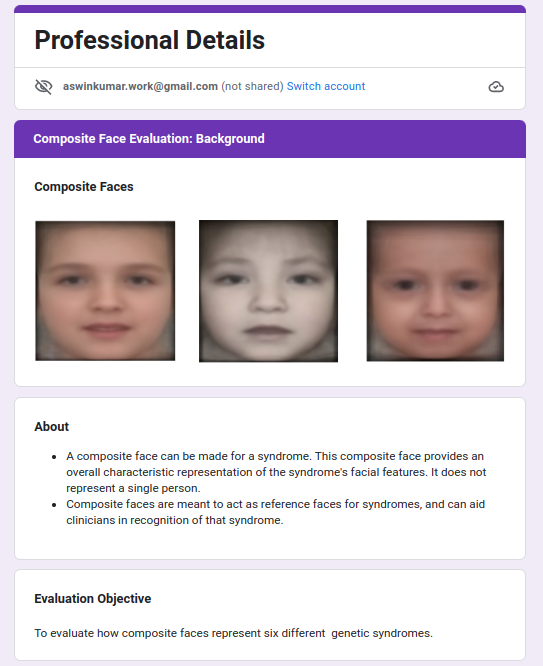
\includegraphics[scale=0.55]{images/quest/3.png}
			\caption{Introduction to the composite face section}
			\addtocounter{figure}{1}
			\label{fig_x}
		\end{figure}
		}
	
	
		\begin{figure}[H]
			\centering
			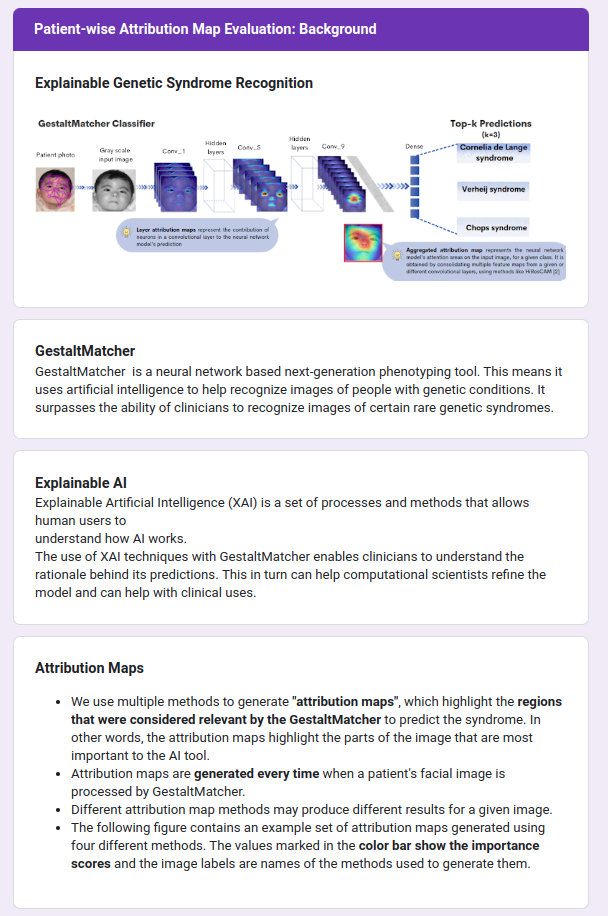
\includegraphics[scale=0.55]{images/quest/4.png}
			\caption{Introduction to the patient-wise attribution map section - part 1}
		\end{figure}
		\begin{figure}
			\continuedfloat
			\centering
			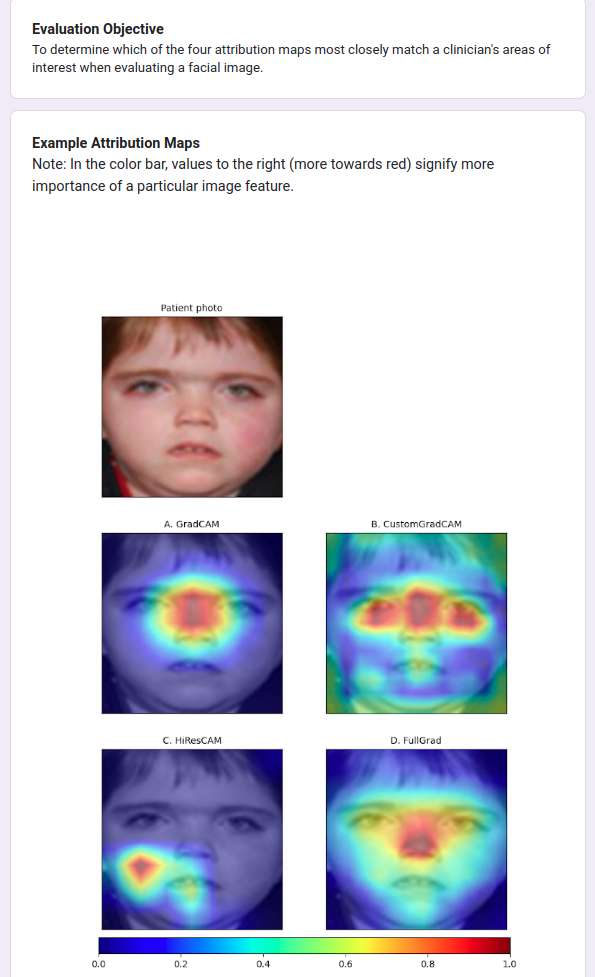
\includegraphics[scale=0.55]{images/quest/5.png}
			\caption{Introduction to the patient-wise attribution map section - part 2}
						\label{fig_y}
			\addtocounter{figure}{1}
		\end{figure}
		
		\begin{figure}[H]
			\centering
			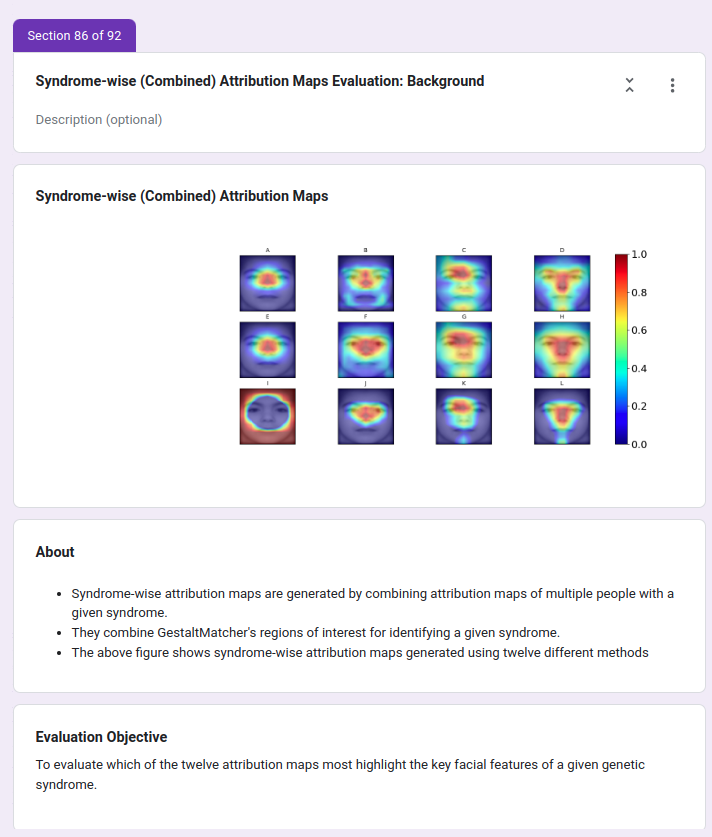
\includegraphics[scale=0.55]{images/quest/6.png}
			\caption{Introduction to the syndrome-wise attribution map section - part 1}
		\end{figure}
		\begin{figure}
			\continuedfloat
			\centering
			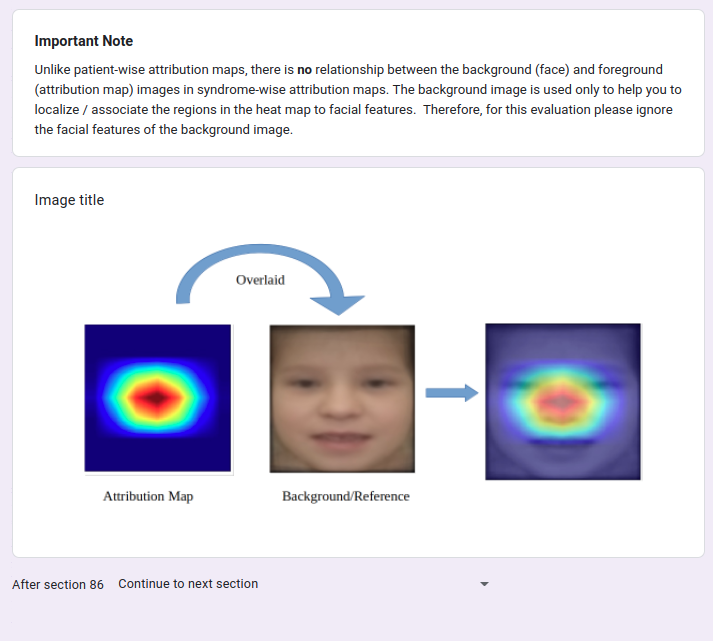
\includegraphics[scale=0.55]{images/quest/7.png}
			\caption{Introduction to the syndrome-wise attribution map section - part 2}
						\label{fig_z}
			\addtocounter{figure}{1}
		\end{figure}
\end{document}
